% --- Template for thesis / report with tktltiki2 class ---
% 
% last updated 2013/02/15 for tkltiki2 v1.02

\documentclass[finnish, grading]{tktltiki2}

% tktltiki2 automatically loads babel, so you can simply
% give the language parameter (e.g. finnish, swedish, english, british) as
% a parameter for the class: \documentclass[finnish]{tktltiki2}.
% The information on title and abstract is generated automatically depending on
% the language, see below if you need to change any of these manually.
% 
% Class options:
% - grading                 -- Print labels for grading information on the front page.
% - disablelastpagecounter  -- Disables the automatic generation of page number information
%                              in the abstract. See also \numberofpagesinformation{} command below.
%
% The class also respects the following options of article class:
%   10pt, 11pt, 12pt, final, draft, oneside, twoside,
%   openright, openany, onecolumn, twocolumn, leqno, fleqn
%
% The default font size is 11pt. The paper size used is A4, other sizes are not supported.
%
% rubber: module pdftex

% --- General packages ---

\usepackage[utf8]{inputenc}
\usepackage[T1]{fontenc}
\usepackage{lmodern}
\usepackage{microtype}
\usepackage{amsfonts,amsmath,amssymb,amsthm,booktabs,color,enumitem,graphicx}
\usepackage[pdftex,hidelinks]{hyperref}
\usepackage{multirow}
\usepackage{tabulary}
\usepackage{float}
\usepackage{enumitem}
%\usepackage{paralist}

\hyphenation{luok-ka-mu-taa-ti-o-o-pe-raat-to-ri}

% Automatically set the PDF metadata fields
\makeatletter
\AtBeginDocument{\hypersetup{pdftitle = {\@title}, pdfauthor = {\@author}}}
\makeatother

% References ilman bracket

\makeatletter 
\renewcommand\@biblabel[1]{#1} 
\makeatother

% --- Language-related settings ---
%
% these should be modified according to your language

% babelbib for non-english bibliography using bibtex
\usepackage[fixlanguage]{babelbib}
\selectbiblanguage{finnish}

% add bibliography to the table of contents
\usepackage[nottoc]{tocbibind}
% tocbibind renames the bibliography, use the following to change it back
\settocbibname{Lähteet}

% --- Theorem environment definitions ---

\newtheorem{lau}{Lause}
\newtheorem{lem}[lau]{Lemma}
\newtheorem{kor}[lau]{Korollaari}

\theoremstyle{definition}
\newtheorem{maar}[lau]{Määritelmä}
\newtheorem{ong}{Ongelma}
\newtheorem{alg}[lau]{Algoritmi}
\newtheorem{esim}[lau]{Esimerkki}

\theoremstyle{remark}
\newtheorem*{huom}{Huomautus}


% --- tktltiki2 options ---
%
% The following commands define the information used to generate title and
% abstract pages. The following entries should be always specified:

\title{Mutaatiotestaus oliojärjestelmissä}
\author{Eveliina Pakarinen}
\date{\today}
\level{Aine}
\abstract{Olioperustaisen ohjelmoinnin kehityksen myötä testausmenetelmiä on sopeutettu uusiin vaatimuksiin, joita olio-ohjelmoinnin erityispiirteet ovat tuoneet mukanaan. Mutaatiotestaus on virheperustainen testausmenetelmä, jonka avulla ohjelmiston olemassa olevien testien laatua voidaan kehittää ja parantaa. Mutaatiotestaus esiteltiin ensimmäistä kertaa jo 1970-luvulla.

Perinteisesti mutaatiotestausta on käytetty testien kehittämisessä proseduraalisella ohjelmoinnilla tuotetuille ohjelmille. Olioperustaisten ohjelmien mutaatiotestaukseen on kuitenkin kehitetty luokkamutaatioksi kutsuttu mutaatiotestausmenetelmä. Mutaatiotestaukseen liittyy ratkaisemattomia ongelmia, jotka estävät mutaatiotestauksen laajamittaisen käytön osana ohjelmistotestausta. 
\vspace{1\baselineskip}\vspace{-\parskip}\\ACM Computing Classification System (CCS):
\\D.2.4 [Software/Program Verification]
\\D.2.5 [Testing and Debugging]
\\D.3.3 [Language Constructs and Features]}

% The following can be used to specify keywords and classification of the paper:

\keywords{mutaatiotestaus, oliojärjestelmät, Java}

% classification according to ACM Computing Classification System (http://www.acm.org/about/class/)
% This is probably mostly relevant for computer scientists
% uncomment the following; contents of \classification will be printed under the abstract with a title
% "ACM Computing Classification System (CCS):"
% \classification{}

% If the automatic page number counting is not working as desired in your case,
% uncomment the following to manually set the number of pages displayed in the abstract page:
%
% \numberofpagesinformation{16 sivua + 10 sivua liitteissä}
%
% If you are not a computer scientist, you will want to uncomment the following by hand and specify
% your department, faculty and subject by hand:
%
% \faculty{Matemaattis-luonnontieteellinen}
% \department{Tietojenkäsittelytieteen laitos}
% \subject{Tietojenkäsittelytiede}
%
% If you are not from the University of Helsinki, then you will most likely want to set these also:
%
% \university{Helsingin Yliopisto}
% \universitylong{HELSINGIN YLIOPISTO --- HELSINGFORS UNIVERSITET --- UNIVERSITY OF HELSINKI} % displayed on the top of the abstract page
% \city{Helsinki}
%


\begin{document}

% --- Front matter ---

\frontmatter      % roman page numbering for front matter

\maketitle        % title page
\makeabstract     % abstract page

\tableofcontents  % table of contents

% --- Main matter ---

\mainmatter       % clear page, start arabic page numbering

% Write some science here.

% Tähän tekstiä. \\ Esimerkki lähdeviitteestä: ~\cite{toinen}.

%\[\frac{a}{b}\]

\section{Johdanto}

Perinteisiä ohjelmistojen testausmenetelmiä on olioperustaisen ohjelmoinnin kehityksen myötä sopeutettu uusiin olio-ohjelmoinnin mukana tuleviin haasteisiin. Olio-ohjelmoinnin avulla voidaan ratkaista joitakin proseduraalisen ohjelmoinnin ongelmia~\cite[s. 86]{Mariani:Pezze:2008}. Olio-ohjelmoinnin piirteet, kuten kapselointi ja perintä, aiheuttavat kuitenkin uusia ongelmia.

Ohjelmistokehitysprosessissa testausta voidaan käyttää ohjelmistossa olevien virheiden havaitsemiseen jo kehitysvaiheen aikana. Testauksen avulla voidaan myös parantaa ohjelmiston laatua ja varmistaa, että ohjelma toimii sille asetettujen vaatimusten mukaisesti. 

Testaukseen liittyy kuitenkin myös rajoituksia. Testauksen avulla ei esimerkiksi voi aina todistaa ohjelmiston oikeellisuutta~\cite[s. 58]{Binder:1999}. Lisäksi epävarmuutta liittyy käytettävän testausjärjestelmän oikeellisuuden ja luotettavuuden varmistamiseen.

Yksi menetelmä ohjelmiston testien laadukkuuden tutkimiseen ja parantamiseen on mutaatiotestauksen käyttö osana ohjelmiston testausprosessia. Mutaatiotestauksessa tavoitteena on tutkia, ovatko ohjelmistoa varten tehdyt testit laadukkaita ja havaitaanko niillä kattavasti ohjelmistossa mahdollisesti esiintyvät virheet ja ongelmat~\cite[s. 649]{Jia:Harman:2011}. 

Mutaatiotestauksen periaatteena on simuloida ohjelmoijien tekemiä yleisiä ohjelmointivirheitä muokkaamalla ohjelmiston alkuperäistä lähdekoodia~\cite[s. 649]{Jia:Harman:2011}. Mutaatiotestauksessa lähdekoodista muodostetaan muunnettuja versioita eli mutantteja. 

Perinteisesti mutaatiotestausta on käytetty testien kehityksessä proseduraalisella ohjelmoinnilla tuotetuille ohjelmille. Olioperustaisen ohjelmoinnin kehittyessä mutaatiotestausta on sopeutettu uusiin vaatimuksiin. Luokkamutaation avulla mutaatiotestausta voidaan soveltaa olio-ohjelmissa testien laadun varmistamiseen~\cite{Kim:Clark:McDermid:2000}.

Vaikka mutaatiotestausta voidaan käyttää apuna ohjelmiston olemassa olevien testien kehittämisessä, liittyy mutaatiotestausmenetelmän käyttöön myös ratkaisemattomia ongelmia, jotka estävät mutaatiotestauksen laaja-alaisen käytön~\cite[s. 652]{Jia:Harman:2011}. Mutaatiotestauksen suoritus vaatii paljon laskentatehoa, mikä on yksi ongelmista. Lisäksi mutaatiotestausprosessissa ihmisiltä vaadittava työpanos on suuri. 

Mutaatiotestausta on tutkittu paljon~\cite[s. 649]{Jia:Harman:2011}. Tutkimuksen avulla on etsitty keinoja ratkaista mutaatiotestaukseen liittyviä ongelmia, jotta mutaatiotestaus voidaan muuttaa käytännölliseksi testausmenetelmäksi. 

%\textcolor{cyan}{Tutkimuskysymys: On tutkittu, että mutaatiotestauksesta on hyötyä testien laadun parantamisessa ja testikattavuuden tarkastelussa/kasvattamisessa. Miksi mutaatiotestausta ei kuitenkaan käytetä laajasti näiden asioiden tekemiseen?}
%
%\textcolor{red}{Vastaus: Koska mutaatiotestaus on tällä hetkellä vielä työlästä ja tehotonta sen tuomaan hyötyyn nähden. Koska mutaatiotestauksessa on ratkaisemattomia ongelmia (esim. ekvivalentit mutantit), joita ei voi automatisoida --> vaativat ihmisten panostusta --> lisää työläyttä.} 
%
%\textcolor{blue}{Tai toisinpäin: Miksi mutaatiotestausta käytettäisiin/pitäisi käyttää enemmän testaamiseen, vaikka mutaatiotestaus on tehotonta/työlästä?}
%
%\textcolor{red}{Vastaus: Koska mutaatiotestausta voidaan käyttää testien laadun parantamiseen tai testikattavuuden kasvattamiseen. Koska mutaatiotestauksen avulla voi varmistaa, että testien laatu on hyvä ja näin ollen parantaa samalla ohjelmiston laatua --> ohjelmistosta saadaan suurin osa ongelmista ja virheistä pois testien avulla. Koska mutaatiotestauksella voi paikata normaaliin testaukseen jääneitä puutteita.} 

%Ohjelmistoja voidaan testata monella tasolla. Testauksen tasot muodostetaan määrittämällä joukko ohjelman osia eli komponentteja, joita halutaan testata. Alimmalla testauksen tasolla testattavat ohjelman osat ovat pienimpiä mahdollisia suoritettavissa olevia komponentteja. Tämän tason testausta kutsutaan \textit{yksikkötestaukseksi} (\textit{unit testing}) ja testattavat osat ovat olio-ohjelmissa esimerkiksi yksittäisiä metodeja tai luokkia~\cite[s. 45]{Binder:1999}.
%
%Yksikkötestauksesta seuraava taso ylöspäin on \textit{integraatiotestaus} (\textit{integration testing}), jossa tarkastellaan järjestelmän tai sen osien yhteistoimintaa ja keskinäistä kommunikointia testaamalla osien välisiä rajapintoja. Olio-ohjelmissa luokkien muodostuminen perinnän avulla ja luokkien koostuminen toisten luokkien olioista aiheuttaa sen, että integraatiotestaukselle on tarvetta jo olioperustaisen ohjelmoinnin alkuvaiheessa~\cite[s. 45]{Binder:1999}.
%
%Valmista integroitua sovellusta testataan \textit{järjestelmätestauksen} (\textit{system testing}) avulla. Tällä testauksen tasolla keskitytään vain valmiissa sovelluksessa esiintyvien piirteiden testaamiseen. Testauksen kohteena voi olla esimerkiksi sovelluksen toiminnallisuus, suorituskyky tai sovelluksen kestämä kuormitus~\cite[s. 45]{Binder:1999}.
%
%Testien suunnittelussa ja kehittämisessä voidaan myös käyttää erilaisia suunnittelumalleja, joiden avulla kuvataan testien suunnitteluun käytettävää näkökulmaa. Ohjelman sisäiseen rakenteeseen eli lähdekoodin tuntemukseen perustuvaa testien suunnittelumallia kutsutaan \textit{white box -testaukseksi}. \textit{Black box -testaukseksi} tai \textit{funktionaaliseksi testaukseksi} kutsutussa suunnittelumallissa testejä suunnitellaan analysoimalla ohjelmiston ulkoista toiminnallisuutta~\cite[s. 52]{Binder:1999}.

%Mutanttien generoinnin jälkeen ohjelmiston alkuperäiset testit suoritetaan jokaisen mutantin kohdalla. Tavoitteena on, että testien avulla havaitaan lähdekoodiin tehdyt muutokset. Jos alkuperäiset testit eivät mene läpi, se tarkoittaa, että mutantti on tapettu eli lähdekoodiin tehdyt muutokset on havaittu~\cite[s. 9]{Kim:Clark:McDermid:2000}. 
%
%Mutaatiotestausprosessi tuottaa lopputuloksena \textit{mutaatiopistemäärän} (\textit{mutation adequacy score}), jonka avulla voidaan arvioida ohjelmiston testien laadukkuutta ja kykyä havaita lähdekoodissa olevia vikoja. 


%\textbf{Johdanto jäsennelty asianmukaisesti (kenelle, miksi, millaisessa ympäristössä; ratkaisun lähestymistapa; tutkimuskysymys, tulokset ja impakti), pituus 1,5 - 2 s.}

%\textbf{\textit{MIKÄ ON MINUN TUTKIMUSKYSYMYKSENI?}}


\section{Testaus oliojärjestelmissä}

Olioperustaisen ohjelmoinnin kehityksen myötä klassisia ohjelmistojen testausmenetelmiä on sopeutettu mahdollistamaan \textit{oliojärjestelmien} (\textit{object oriented systems}) kattava ja laadukas testaaminen. Vaikka olioperustainen ohjelmointi ratkaisee joitakin proseduraalisen ohjelmoinnin suunnittelu- ja toteutusongelmia, olio-ohjelmoinnin mukana tulevat uudet haasteet vaativat uusien testaus- ja analysointimenetelmien kehittämistä~\cite[s. 86]{Mariani:Pezze:2008}. 

\subsection{Testauksen rooli oliojärjestelmissä}

Testausta käytetään ohjelmistokehityksessä ohjelmiston laadun varmistamiseen ja auttamaan virheiden havaitsemisessa jo kehitysvaiheen aikana. Ohjelmistojen testaamisen ensisijainen tavoite on siis paljastaa virheitä, joiden havaitseminen muiden laadunvarmistusmenetelmien avulla olisi työlästä tai mahdotonta~\cite[s. 59]{Binder:1999}. Testauksen avulla pyritään lisäksi varmistamaan, että ohjelma toimii sille asetettujen vaatimusten mukaisesti. 

Olio-ohjelmoinnissa testaukseen tuovat haasteita olio-ohjelmien erityispiirteet, joita ovat muun muuassa kapselointi, perintä, dynaaminen sidonta ja polymorfismi~\cite[s. 86]{Mariani:Pezze:2008}. 
\textbf{Lisää tähän? Binderin kirjasta löyty tietoa.}


\subsection{Testauksen tasot}

Ohjelmistoja voidaan testata usealla tasolla. Testauksen tasoja ovat yksikkö-, integraatio- ja järjestelmätasot. Tasot muodostuvat yhdestä tai useammasta ohjelman komponentista, joita tason testeillä testataan~\cite[s. 45]{Binder:1999}. Komponentti voi olio-ohjelmissa olla esimerkiksi yksittäinen metodi tai luokka, ohjelman luokkien välinen rajapinta tai jo valmis ohjelmisto.

Alimmalla testauksen tasolla \textit{yksikkötestauksessa} (\textit{unit testing}) testataan ohjelman pienimpiä suoritettavissa olevia komponentteja~\cite[s. 45]{Binder:1999}. Olio-ohjelmissa näitä komponentteja ovat yksittäiset metodit ja oliot. 
\textbf{Lisää tietoa yksikkötestauksesta.}

Yksikkötestauksesta seuraava taso ylöspäin on \textit{integraatiotestaus} (\textit{integration testing}), jossa tarkastellaan järjestelmän tai sen osien yhteistoimintaa~\cite[s. 45]{Binder:1999}. Integraatiotestauksessa testataan siis järjestelmän osien välisiä rajapintoja ja osien keskinäistä kommunikointia. Olio-ohjelmissa luokkien muodostumisesta perinnän avulla ja luokkien koostumisesta toisten luokkien olioista seuraa, että integraatiotestaukselle on olio-ohjelmoinnissa tarvetta jo ohjelmoinnin alkuvaiheessa. 
\textbf{Lisää ehkä vähän myös tästä.}

Valmista integroitua sovellusta testataan \textit{järjestelmätestauksen} (\textit{system testing}) avulla~\cite[s. 45]{Binder:1999}. Tällä testauksen tasolla keskitytään vain valmiissa sovelluksessa esiintyvien piirteiden testaamiseen. Testauksen kohteena voi olla esimerkiksi sovelluksen toiminnallisuus, suorituskyky tai sovelluksen kestämä kuormitus~\cite[s. 45]{Binder:1999}. 
\textbf{Tästä jonkin verran lisää.}

\textbf{Joku kokoelmakuva testauksen tasoista + testausmenetelmistä?}

\subsection{Testien suunnittelu}

Testien suunnitteluun ja kehittämiseen voidaan käyttää useita menetelmiä. Testausmenetelmän avulla kuvataan näkökulmaa, josta esimerkiksi ohjelman lähdekoodia tarkastellaan testejä kehitettäessä~\cite[s. 51]{Binder:1999}. Uusia testejä kehitettäessä testausmenetelmiä ovat esimerkiksi white box -testaus ja black box -testaus sekä niitä yhdistävä hybriditestaus. Virheisiin perustuvan testausmenetelmän avulla voidaan kehittää olemassa olevia testejä.

Ohjelman sisäisen rakenteen eli lähdekoodin tuntemukseen perustuvaa testausmenetelmää kutsutaan \textit{white box -testaukseksi}~\cite[s. 52]{Binder:1999}. \textbf{Lisää tästä.} White box -testausta voidaan käyttää esimerkiksi yksikkötestauksessa apuna testien suunnittelussa, sillä lähdekoodin tuntemus auttaa kehittämään testejä yksittäisille metodeille ja olioille.

\textit{Black box -testaukseksi} eli \textit{funktionaaliseksi testaukseksi} kutsutussa testausmenetelmässä testejä suunnitellaan ohjelmiston toiminnallisuuden tuntemuksen avulla~\cite[s. 52]{Binder:1999}. \textbf{Lisää tuosta.} Koska valmiin sovelluksen piirteitä testattaessa tutkitaan myös sovelluksen ulkoista toiminnallisuutta, on black box -testausmenetelmästä apua suunniteltaessa testejä esimerkiksi järjestelmätestaukseen.

\textit{Gray box -} eli \textit{hybriditestauksessa} yhdistetään white box - ja black box -testausmenetelmien piirteitä~\cite[s. 52]{Binder:1999}. Sekä white box - että black box -testausmenetelmää voidaan käyttää testien suunnittelussa useilla testauksen tasoilla joko erikseen tai molempien piirteitä yhdistäen.

Testausmenetelmää, jossa ohjelman lähdekoodiin lisätään virheitä, kutsutaan \textit{virheperustaiseksi testausmenetelmäksi} (\textit{fault-based testing})~\cite[s. 52]{Binder:1999}. Esimerkkinä virheperustaisesta testausmenetelmästä on mutaatiotestaus, jonka avulla tutkitaan testien kykyä havaita ohjelmistossa olevia virheitä~\cite[s. 36]{DeMillo:Lipton:Sayward:1978}. Testaukseen liittyvät tavoitteet ovat mutaatiotestauksessa ja perinteisessä ohjelmistotestauksessa toistensa vastakohtia. Perinteisessä testauksessa keskitytään parantamaan ohjelmiston laatua, kun taas mutaatiotestauksessa kehityksen kohteena ovat olemassa olevat testit ja niiden laatu.

\subsection{Testauksen rajoitukset}

Yksi testaukseen liittyvistä rajoituksista on, että testauksen avulla ei voi aina todeta ohjelmiston oikeellisuutta. Jotta oikeellisuus voidaan todistaa, vaaditaan, että ohjelman oikea toiminta testataan kaikilla mahdollisilla syötteillä ja niiden kombinaatioilla. Ohjelman oikeellisuuden todistaminen vastaa siis ohjelman kattavaa testaamista. Kattava testaaminen on kuitenkin käytännössä usein mahdotonta toteuttaa muille kuin triviaaleille ohjelmille~\cite[s. 58]{Binder:1999}. Oikellisuuden todistamiseen liittyen Edsger Dijkstra totesikin: \textit{''Program testing can be used to show the presence of bugs, but never to show their absence!''}~\cite[s. 6]{Dahl:Dijkstra:Hoare:1972}.

Suoritettujen testien tulosten tulkintaan liittyy myös rajoituksia ja epävarmuutta. Epävarmuus ilmenee, kun testien suorituksen tuloksia varten ei ole olemassa  vertailukohdaksi luotettavia odotettuja tuloksia. Tällöin testauksesta saatujen toteutuneiden tulosten tulkinta ja arviointi on epävarmaa. Toteutuneista tuloksista ei voi siis luotettavasti päätellä, menivätkö testit läpi vai eivät~\cite[s. 58]{Binder:1999}. 

Epävarmuutta liittyy myös testattavan järjestelmän halutulle toiminnallisuudelle asetettuihin vaatimuksiin. Toiminnallisuusvaatimusten todentaminen testauksen avulla ei ole mahdollista, joten vaatimuksia on käytettävä vain vertailukohtana testauksen tulosten tulkinnassa~\cite[s. 58]{Binder:1999}. Jos virheellisiä tai puutteellisia vaatimuksia käytetään testejä tehdessä, voi siitä seurata harhaanjohtavia testejä. Testauksen avulla ei myöskään voi paljastaa lähdekoodista puuttuvia osia, sillä olematonta koodia ei voi testata~\cite[s. 58]{Binder:1999}.

\textbf{Rajoituksista selvennettävä noita 2 viimeistä kappaletta. Niissä voi olla jotakin epäselvyyksiä. Ainakin mulla vielä on joten vois selventää niitä huvin vuoksi.}

\section{Mutaatiotestaus}

Testaukseen sisältyvien rajoitusten lisäksi testaukseen liittyy myös epävarmuutta käytettävän testausjärjestelmän oikeellisuudesta ja oikeellisuuden varmistamisesta~\cite[s. 209]{Manna:Waldinger:1978}. Tämä herättää kysymyksen siitä, kuka voi ''valvoa valvojia'' eli kuinka varmistetaan ohjelmiston testien laadukkuus. Yksi mahdollisuus testien kehittämiseen ja niiden laadun parantamiseen on \textit{mutaatiotestaus}. Mutaatiotestauksen avulla voidaan mitata, kuinka tehokkaasti ohjelmiston testeillä havaitaan ohjelmistossa esiintyviä virheitä~\cite[s. 649]{Jia:Harman:2011}.

\subsection{Mutaatiotestauksen historia ja periaatteet/teoreettinen perusta}

Mutaatiotestauksesta kirjoitettiin ensimmäistä kertaa jo 1970-luvulla. Richard DeMillon, Richard Liptonin ja Frederick Saywardin artikkeli~\cite{DeMillo:Lipton:Sayward:1978} vuodelta 1978 on yksi ensimmäisistä uraauurtavista mutaatiotestausta esittelevistä artikkeleista. Mutaatiotestauksen tutkimus on lisääntynyt vuosien kuluessa, ja erityisesti 2000-luvulla uusia tuloksia on julkaistu paljon~\cite[s. 1102]{Offutt:2011}. Tutkimuksessa suuntana on ollut etsiä keinoja, joilla mutaatiotestaus voidaan muuttaa käytännölliseksi testausmenetelmäksi~\cite[s. 649]{Jia:Harman:2011}. 

\textbf{historiasta ehkä lisää ja tutkimuksesta}

Mutaatiotestaus perustuu kahteen hypoteesiin: the Competent Programmer Hypothesis ja the Coupling Effect (Hypothesis).

\textbf{Lisää juttua siitä, että mutaatiotestaus kasvattaa testitkattavuutta.}

\subsection{Perinteinen mutaatiotestausprosessi}

Perinteisessä mutaatiotestausprosessissa prosessin \textbf{lähtökohtina/ lähtökohtana} ovat ohjelmisto ja ohjelmistoa varten tehdyt testit. Perinteisen mutaatiotestauksen aikana olemassa olevien testien laatua kehitetään vaiheittain. Perinteisen mutaatiotestausprosessin työvaiheet on esitelty kuvassa \ref{figure:Mutaatiotestausprosessi}. Työvaiheet on merkitty kuvaan sinisillä \textbf{laatikoilla}. Työvaiheiden aikana käytettäviä resursseja, \textbf{kuten esimerkiksi} ohjelmiston lähdekoodia ja testituloksia, kuvataan vihreillä ja keltaisilla laatikoilla. \textbf{Mihin kuva sijoitetaan?}

Perinteisessä mutaatiotestausprosessissa ensimmäinen vaihe on käsitellä ohjelmiston alkuperäistä lähdekoodia \textit{mutaatio-operaattoreilla}, jotka muuntavat koodia muodostaen siitä virheellisiä versioita~\cite[s. 869]{Ma:Harrold:Kwon:2006}. Näitä virheellisiä ohjelmakoodin versioita kutsutaan \textit{mutanteiksi}. Mutaatio-operaattorit kuvaavat algoritmeja, joiden avulla lähdekoodia käsitellään koodin muuntamisen aikana.

Mutanttien generoinnin jälkeen ohjelmiston alkuperäiset testit suoritetaan muuntamattomalle lähdekoodille~\cite[s. 652]{Jia:Harman:2011}. Tavoitteena on varmistaa, että testit voidaan suorittaa alkuperäiselle ohjelmalle ilman virheitä. Jos testit eivät mene läpi eli ohjelmassa havaitaan virheitä, virheet korjataan ennen kuin mutaatiotestausta jatketaan. 

Seuraavaksi testit suoritetaan jokaisen elävän mutantin kohdalla~\cite[s. 35]{Offutt:Untch:2001}. Mutanttien testaamisen tavoitteena on selvittää, havaitaanko testien avulla lähdekoodiin tehdyt muutokset. 

Testien suorituksen jälkeen suorituksesta saatuja tuloksia verrataan toisiinsa. Testituloksia vertailtaessa voidaan päästä kahteen lopputulokseen~\cite[s. 36]{DeMillo:Lipton:Sayward:1978}. Alkuperäiselle muuntamattomalle lähdekoodille suoritettujen testien tulos voi: 
\begin{enumerate}
  \item erota yhdelle mutantille suoritettujen testien tuloksesta tai
  \item olla sama kuin yhdelle mutantille suoritettujen testien tulos.
\end{enumerate}

Tapauksessa 1. alkuperäiset testit eivät ole menneet läpi mutantin kohdalla. Tämä tarkoittaa, että mutantti on tapettu eli lähdekoodiin tehty muutos on havaittu~\cite[s. 36]{DeMillo:Lipton:Sayward:1978}.

Tapauksessa 2. alkuperäiset testit ovat menneet läpi mutantin kohdalla eli mutantti on jäänyt eloon. Mutantin jäämiselle eloon on kaksi vaihtoehtoista selitystä~\cite[s. 36]{DeMillo:Lipton:Sayward:1978}. Ensimmäinen selitys on, että alkuperäiset testit eivät ole riittävän hyvät, jotta niiden avulla voidaan havaita lähdekoodiin tehty muutos. Toinen selitys on, että mutantin toiminta ei eroa alkuperäisen ohjelman toiminnasta eli kyseessä on \textit{ekvivalentti mutantti}. Ekvivalentti mutantti on syntaktisesti erilainen kuin alkuperäinen ohjelma mutta toiminnaltaan se on samanlainen alkuperäisen ohjelman kanssa~\cite[s. 652]{Jia:Harman:2011}.

Jos testituloksia verrattaessa huomataan, että mutantteja on jäänyt eloon, seuraava vaihe mutaatiotestausprosessissa on etsiä ja merkitä ekvivalentit mutantit~\cite[s. 36]{Offutt:Untch:2001}. Tämän jälkeen testien laatua voidaan kehittää joko muokkaamalla olemassa olevia testejä tai lisäämällä uusia testejä, jotta \textbf{eloon jääneet (yhteen/erikseen?)} mutantit saadaan tapettua.

Mutaatiotestausprosessi tuottaa lopputuloksena \textit{mutaatiopistemäärän} (\textit{mutation adequacy score}), jonka avulla voi arvioida ohjelmiston testien laadukkuutta ja kykyä havaita lähdekoodissa olevia vikoja~\cite[s. 652]{Jia:Harman:2011}. Mutaatiopistemäärä \textit{MP} lasketaan kaavalla 
\begin{equation}
MP = \frac{T}{K - E},
\end{equation}
missä \textit{T} on tapettujen mutanttien määrä, \textit{K} on kaikkien mutanttien määrä ja \textit{E} on ekvivalenttien mutanttien määrä. Mutaatiopistemäärän maksimiarvo 1 saavutetaan, kun testeillä saadaan tapettua kaikki mutantit~\cite[s. 36]{Offutt:Untch:2001}. Testit ovat tällöin \textit{\textbf{adequate relative to the mutants}} riittävät havaitsemaan kaikki mutantit. Perinteinen mutaatiotestausprosessi päättyy, kun kaikki \textbf{\textit{ei-ekvivalentit} (miten tämä kirjoitetaan?)} mutantit on tapettu. Tämä on merkitty kuvaan \ref{figure:Mutaatiotestausprosessi} violetilla laatikolla.

\begin{figure}[H]
	\centering
		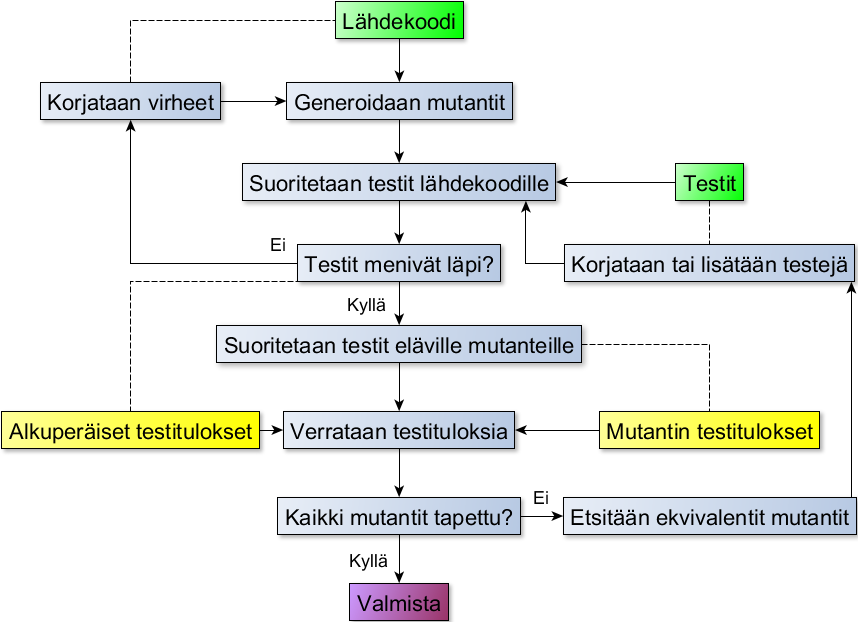
\includegraphics[width=\textwidth]{mutaatiotestausprosessi2}
	\caption{Perinteinen mutaatiotestausprosessi.}
	\label{figure:Mutaatiotestausprosessi}
\end{figure}

\subsection{Uusi mutaatiotestausprosessi}

\textbf{Onko tämä hyvä omana kappaleenaan vai voiko tai pitääkö laittaa perinteisen prosessin loppuun? Omaa muotoilua perustuen Uniting orthogonal 2000 artikkeliin --> uusi mutaatiotestausprosessi:} Kuvasta \ref{figure:Mutaatiotestausprosessi} huomataan, että perinteinen mutaatiotestausprosessi sisältää silmukoita. Ensimmäinen silmukka sisältää mutanttien generoinnin, testien suorituksen alkuperäiselle lähdekoodille ja testien tulosten tarkastamisen jälkeen virheiden korjauksen. Näistä työvaiheista alkuperäisten testitulosten tarkastaminen ja alkuperäisen ohjelman virheiden korjaaminen vaativat manuaalista työtä.

Toinen silmukka eli mutaatiotestauksen pääsilmukka muodostuu työvaiheista, jotka suoritetaan alkuperäisten testitulosten läpimenotarkastuksen jälkeen. Toiseen silmukkaan sisältyvät myös ensimmäisen silmukan työvaiheista testien suoritus lähdekoodille ja testien läpimenotarkastus. Tämä tarkoittaa, että silmukat risteävät näiden työvaiheiden kohdalla. Toisessa silmukassa manuaalista työtä vaativat ekvivalenttien mutanttien etsiminen ja merkitseminen ja uusien testien lisääminen tai olemassa olevien testien kehittäminen.

\textbf{En tiedä, onko tämä uusi prosessi jo käytössä?} Jotta perinteistä mutaatiotestausprosessia voidaan tehostaa, manuaaliset työvaiheet on poistettava mutaatiotestauksen pääsilmukasta~\cite[s. 41]{Offutt:Untch:2001}. Tällöin perinteisen mutaatiotestausprosessin tilalle muodostuu uusi testausprosessi, jossa osa työläistä manuaalisista työvaiheista suoritetaan automaattisesti. 

Automatisoitavia työvaiheita uudessa mutaatiotestausprosessissa ovat ekvivalenttien mutanttien tunnistaminen ja testien generointi ja kehittäminen. Ainoaksi merkittäväksi manuaaliseksi työvaiheeksi jää tarkistaa, ovatko alkuperäiselle lähdekoodille suoritetut testit menneet läpi. Jotta alkuperäisen lähdekoodin testitulosten tarkastusvaihe saadaan pois mutaatiotestauksen pääsilmukasta, suoritetaan läpimenotarkastus uudessa mutaatiotestausprosessissa pääsilmukasta poistuttaessa. Työvaiheiden automatisointi ja niiden suoritusjärjestyksen muuttaminen tekevät uudesta mutaatiotestausprosessista tehokkaamman verrattuna perinteiseen mutaatiotestausprosessiin~\cite[s. 41]{Offutt:Untch:2001}.

\section{Mutaatiotestaus oliojärjestelmissä}

Kappaleen estittelyteksti tähän. \textbf{Kuinka pitkä tämän on oltava?} 

\subsection{Mutaatiotestauksen piirteet oliojärjestelmissä}

MuJava-artikkelista --> inter-intra/class-method testaus.

\subsection{Mutaatio-operaattorit oliojärjestelmissä}

Mutaatio-operaattorit ovat tärkeässä asemassa mutaatiotestauksessa, sillä mutaatiotestauksen tehokkuus riippuu siitä, minkälaisia virheitä mutaatio-operaattoreilla luodaan lähdekoodiin~\cite[s. 352]{Ma:Kwon:Offutt:2002}. Perinteisesti mutaatiotestausta on hyödynnetty proseduraalisessa ohjelmoinnissa, minkä vuoksi myös mutaatio-operaattorit on kehitetty tukemaan suurinta osaa proseduraalisten ohjelmointikielten piirteistä~\cite[s. 352]{Ma:Kwon:Offutt:2002}. 

Olioperustaisiin ohjelmointikieliin sisältyy kuitenkin uusia ominaisuuksia, joiden käytöstä aiheutuu erilaisia virheitä verrattuna proseduraalisessa ohjelmoinnissa esiintyviin virheisiin. Uusien virheiden ilmeneminen olio-ohjelmissa on johtanut uusien olioperustaisten mutaatio-operaattorien kehittämiseen.  

Olioperustaisten ohjelmien mutaatiotestaukseen käytettävää menetelmää kutsutaan \textit{luokkamutaatioksi}~\cite{Kim:Clark:McDermid:2000}. Luokkamutaatiomenetelmän kehittivät Sunwoo Kim, John Clark ja John McDermid Java-oh\-jel\-moin\-ti\-kie\-les\-sä esiintyvien virheiden pohjalta~\cite{Kim:Clark:McDermid:2000}. Heidän kehittämiensä \textit{luokkamutaatio-operaattorien} avulla mutaatiotestausmenetelmää voidaan soveltaa Java-ohjelmointikielellä toteutettuihin olioperustaisiin ohjelmiin.

Kimin, Clarkin ja McDermidin kehittämät luokkamutaatio-operaattorit ovat toimineet lähtökohtana myös muiden tutkijoiden luokkamutaatiotutkimuksessa ja uusien luokkamutaatio-operaattorien kehittämisessä. Yu Seung Ma, Yong Rae Kwon ja Jeff Offutt kehittivät vuonna 2002 Java-oh\-jel\-moin\-ti\-kiel\-tä varten joukon uusia luokkamutaatio-operaattoreita, jotka perustuivat aiemmin kehitettyihin operaattoreihin~\cite[s. 352]{Ma:Kwon:Offutt:2002}. Heidän tavoitteenaan oli parantaa ja kehittää olemassa olevia luokkamutaatio-operaattoreita, jotta luokkien välisten suhteiden testaaminen olisi mahdollista mutaatiotestauksella~\cite[s. 362]{Ma:Kwon:Offutt:2002}.

Taulukossa \ref{table:Mutaatio-operaattorit-taulukko} on listattu Man, Kwonin ja Offuttin kehittämät luok\-ka\-mu\-taa\-ti\-o-o\-pe\-raat\-to\-rit. Operaattorit on jaettu kuuteen ryhmään. Ryhmät perustuvat niihin olio-ohjelmointikielen piirteisiin, joita ryhmän operaattoreilla muunnetaan~\cite[s. 355]{Ma:Kwon:Offutt:2002}.

Mutaatio-operaattorien avulla kuvataan algoritmeja, joilla lähdekoodia muokataan mutantteja muodostettaessa. Esimerkiksi JSC-operaattori lisää ilmentymämuuttujiin \textit{static}-määreen tehden niistä luokkamuuttujia tai vastaavasti poistaa luokkamuuttujista \textit{static}-määreen tehden niistä ilmentymämuuttujia. JSC-operaattorin ja myös muiden Man, Kwonin ja Offuttin kehittämien luokkamutaatio-operaattorien nimet ja kuvaukset voi nähdä taulukosta \ref{table:Mutaatio-operaattorit-taulukko}. Taulukosta nähdään myös, mihin ryhmiin luokkamutaatio-operaattorit kuuluvat. Tarkemmat tiedot operaattorien toiminnasta löytyvät artikkelista~\cite{Ma:Kwon:Offutt:2002}. 

\begin{table}[H]
\begin{spacing}{1.0}
	\begin{center}
		\centering
		\begin{tabulary}{1\textwidth}{|L|L|L|}
			\hline
			\textbf{Ryhmä} & \textbf{Operaattori} & \textbf{Kuvaus} \\
			\hline
			\parbox[t]{2cm}{Kapselointi} & AMC & Access modifier change \\
			\hline
			\multirow{8}{*}{\parbox[t]{2cm}{Perintä}} & IHD & Hiding variable deletion \\ \cline{2-3}
			& IHI & Hiding variable insertion \\ \cline{2-3}
			& IOD & Overriding method deletion \\ \cline{2-3}
			& IOP & \parbox[t]{7cm}{Overridden method calling position change} \\ \cline{2-3}
			& IOR & Overridden method rename \\ \cline{2-3}
			& ISK & \textit{super} keyword deletion \\ \cline{2-3}
			& IPC & \parbox[t]{7cm}{Explicit call of a parent's constructor deletion} \\
			\hline
			\multirow{7}{*}{\parbox[t]{2cm}{Polymor-\\fismi}} & PNC & \textit{new} method call with child class type \\ \cline{2-3}
			& PMD & \parbox[t]{7cm}{Member variable declaration with parent class type} \\ \cline{2-3}
			& PPD & \parbox[t]{7cm}{Parameter variable declaration with\\child class type}
\\ \cline{2-3}
			& PRV & \parbox[t]{7cm}{Reference assignment with other\\compatible type} \\
			\hline
			\multirow{4}{*}{\parbox[t]{2cm}{Metodin\\ylikuormi-\\tus}} & OMR & Overloading method contents change \\ \cline{2-3}
			& OMD & Overloading method deletion \\ \cline{2-3}
			& OAO & Argument order change \\ \cline{2-3}
			& OAN & Argument number change \\
			\hline 
			\multirow{4}{*}{\parbox[t]{2cm}{Javan\\erityis-\\piirteet}} & JTD & \textit{this} keyword deletion \\ \cline{2-3}
			& JSC & \textit{static} modifier change \\ \cline{2-3}
			& JID & Member variable initialization deletion \\ \cline{2-3}
			& JDC &  \parbox[t]{7cm}{Java-supported default constructor create} \\
			\hline
			\multirow{5}{*}{\parbox[t]{2cm}{Yleiset\\ohjelmoin-\\tivirheet}} & EOA & \parbox[t]{7cm}{Reference assignment and content assignment replacement} \\ \cline{2-3}
			& EOC & \parbox[t]{7cm}{Reference comparison and content comparison replacement} \\ \cline{2-3}
			& EAM & Accessor method change \\ \cline{2-3}
			& EMM & Modifier method change \\
			\hline
		\end{tabulary}
	\end{center}      
	\caption{Luokkamutaatio-operaattoreita Javalle.}
	\label{table:Mutaatio-operaattorit-taulukko}
\end{spacing}
\end{table}


\subsection{Automatisoidut mutaatiojärjestelmät}

MuJava? jotakin muita. Onko yleisessä käytössä olevia (commercial) järjestelmiä?


\section{Mutaatiotestauksen haasteet}

Vaikka mutaatiotestausta voidaan käyttää ohjelmiston olemassa olevien testien kehittämiseen ja testien laadun parantamiseen, ei mutaatiotestausmenetelmän käyttö ole ongelmatonta. Mutaatiotestaukseen liittyy haasteita, jotka estävät menetelmän käyttämisen laaja-alaisesti osana testausprosessia~\cite[s. 652]{Jia:Harman:2011}.

%\textbf{Misi mutaatiotestaus ei ole päätynyt suureen suosioon/käyttöön? Valitaan muutama haaste ja esitellään niitä? Kerrotaan että myös muita haasteita, mutta ei esitellä niitä niin tarkasti?} HAASTEITA ON JAETTAVA TUTKIELMASSA OMIIN ALALUKUIHINSA. NYT TEHDÄÄN VAIN HAASTEITA VARTEN NS. "JOHDANTOKAPPALE" JONKA VOI TUTKIELMASSA JAKAA OMIKSI KAPPALEIKSEEN.

%\textbf{\textit{Haasteet sisältäen esimerkin, miten se yksittäinen haaste on yritetty ratkaista (eli joko ratkaisu tai ratkaisuehdotus)??}}

\subsection{Ekvivalentit mutantit}

\textbf{Ratkaisematon ongelma --> jos sais sen todistukse käsiin?? En tiedä, onko se mahdollista. TODO: Esimerkki ekvivalenteista mutanteista.}

Yleinen ekvivalenttien mutanttien tunnistaminen (tunnistamisongelma) on ratkaisematon by Budd and Angluin \textbf{ETSI LÄHDE}. Heuristiikkoja kehitetty, jotta ongelman voi ratkaista osittain. Compiler optimization techniques, algorithms in Mothra, infeasible constraints ideaan perustuva väline, Program slicing. Estää jo alkuunsa mutantttien syntymisen eikä etsi niitä vasta sitten, kun ne ovat syntyneet.~\cite[s. 79]{Offutt:Ma:Kwon:2006:MuClassLevel}

Toinen mutaatiotestaukseen liittyvistä ongelma-alueista on ekvivalentit mutantit. Ekvivalenttien mutanttien tunnistaminen algoritmien avulla on ratkaisematon ongelma~\cite[s. 657]{Jia:Harman:2011}. Koska ekvivalentteja mutantteja ei voi tunnistaa laskennan avulla, ihmisten on suoritettava ekvivalenttien mutanttien tunnistaminen tutkimalla mutanttia ja vertaamalla sen toimintaa alkuperäisen ohjelmiston toimintaan. Tämä menetelmä johtaa mutaatiotestauksen toteuttamiseen tarvittavan työmäärän kasvuun. Ekvivalenttien mutanttien tunnistamisongelma on kuitenkin herättänyt runsaasti teoreettista kiinnostusta, ja mahdollisia tunnistamistekniikoita on tutkittu paljon~\cite[s. 657]{Jia:Harman:2011}. 

\subsection{Tehokkuusongelmat}

\textit{Do fewer, do smarter, do faster} ovat ratkaisuehdotuksia.~\cite[s. 121]{Ma:Offutt:Kwon:2005:MuAutomated} 

Do smarter laskentatyön jakaminen usealle laitteelle tai weak mutation. 

Do faster mutanttien generoinnin/kääntämisen ja suorituksen tehostaminen, jotta voitaisiin suorittaa niin nopeasti kuin mahdollista. MSG metodi (MuJava) tai compiler-integrated program mutation tai separate compilation.

Do fewer vähemmän mutantteja ilman "mutaatiokattavuuden" kärsimistä suuresti. Mutant sampling, selective mutation, 

Yksi mutaatiotestauksen ongelma-alueista on tehokkuuteen liittyvät ongelmat. Tehokkuusongelmia esiintyy erityisesti silloin, kun jokaisen mutantin kohdalla suoritetaan kaikki ohjelmistoa varten tehdyt testit~\cite[s. 652]{Jia:Harman:2011}. Testien suoritus jokaisen mutantin kohdalla hidastaa mutaatiotestausprosessia ja vaatii paljon laskentatehoa. Tehokkuusongelman ratkaisemiseksi on kuitenkin esitetty useita ratkaisuehdotuksia~\cite[s. 653]{Jia:Harman:2011}. Ratkaisuehdotuksia ovat esimerkiksi generoitujen mutanttien määrän vähentäminen ja mutanttien ja testien suorituskustannusten pienentäminen.

\subsection{Manuaalinen työ}

\textbf{Tähän liittyy ekvivalentit mutantit --> niiden tunnistaminen ja human oracle ongelma --> eli ihmisen käytävä testitulokset läpi sen jälkeen kun tulokset on saatu.}

Kolmas ongelma-alue liittyy mutaatiotestauksen vaiheeseen, jossa ihmisten on tarkastettava testauksesta saadut tulokset~\cite[s. 652]{Jia:Harman:2011}. Tarkastusvaiheessa testien suorituksen jälkeen tarkastetaan suorituksesta saatu tuloste. Tulosteen tarkastusvaihe on usein testausprosessin työläin osa~\cite[s. 653]{Jia:Harman:2011}. Tämä ongelma ei liity pelkästään mutaatiotestaukseen vaan ongelma ilmenee myös muissa testausmenetelmissä. Mutaatiotestauksessa ekvivalenttien mutanttien tunnistaminen ja suoritettujen testien suuri määrä lisäävät kuitenkin työmäärää, joka tarvitaan testauksen tulosten tarkastamiseen.


%__________________________________________________________

%\section{Miten mutaatiotestaus auttaa testien laadun parantamisessa?}

%\subsection{Miksi mutaatiotestausta tulisi käyttää, vaikka se on raskasta ja työlästä?}

%\subsection{Miltä tulevaisuus näyttää, tuleeko käyttö lisääntymään vai jääkö mutaatiotestaus unohduksiin/pienen piirin harrastukseksi?}


\section{Yhteenveto}

Olioperustaisen ohjelmoinnin mukana tulevien uusien haasteiden kohtaaminen vaatii muutoksia myös ohjelmistojen testausmenetelmiin. Sekä perinteisiä olemassa olevia että uusia testausmenetelmiä kehitetään, jotta olio-ohjelmia voidaan testata kattavasti ja laadukkaasti. 

Perinteisessä ohjelmistotestauksessa keskitytään ohjelmiston toiminnallisuuden testaamiseen ja virheiden etsimiseen ohjelmistosta. Perinteiseen ohjelmistotestaukseen liittyy kuitenkin haasteita, jotka aiheuttavat testaukseen epävarmuutta. Yksi haasteista on määrittää, ovatko testauksessa käytettävät testit ja testausjärjestelmä riittävän luotettavia, jotta niiden avulla ohjelmistoa voidaan testata laadukkaasti.

Mutaatiotestaus on virheperustainen testausmenetelmä, joka tarjoaa ratkaisun testien laadun määrittämiseen liittyvään haasteeseen. Mutaatiotestauksen avulla voidaan mitata ohjelmistoa varten tehtyjen testien kykyä havaita ohjelmistossa esiintyviä virheitä. Mutaatiotestausmenetelmän avulla on siis mahdollista kehittää olemassa olevia testejä ja parantaa testien luotettavuutta.

Mutaatiotestauksen käyttö yleisesti osana testausprosessia on vähäistä mutaatiotestaukseen liittyvien ratkaisemattomien ongelmien takia. Mutaatiotestausta on kuitenkin tutkittu paljon. Tutkimuksen avulla voi olla mahdollista löytää ratkaisuja mutaatiotestausta vaivaaviin ongelmiin, jotta mutaatiotestauksen laaja-alainen käyttö voisi tulevaisuudessa olla mahdollista.

%Tällä (yksikkö)testauksen tasolla testien suunnittelussa voidaan käyttää ohjelman sisäiseen rakenteeseen perustuvaa suunnittelumallia, jota kutsutaan \textit{white box -testaukseksi} (\textit{white box testing}). Tässä mallissa ohjelmiston lähdekoodia käytetään apuna testien valmistamisessa~\cite[s. 52]{Binder:1999}.

%Tämän tason testien suunnittelustrategiana voidaan käyttää ohjelmiston ulkoisen toiminnallisuuden analysointia. Tällaista testausstrategiaa kutsutaan \textit{black box -testaukseksi} (\textit{black box testing}) tai \textit{funktionaaliseksi testaukseksi} (\textit{functional testing})~\cite[s. 52]{Binder:1999}. Kuitenkin sekä white box - että black box -testausta voidaan käyttää kaikilla testauksen tasoilla testien suunnittelun apuna. 

%\section{Miten saa evaluointia/analyysiä? Mihin lukuihin se sopii?}

%\textbf{Mihin kohtiin evaluointi ja analyysi sopivat, jotta tästä ei tule mutaatiotestauksen/testauksen oppikirjaa? Miten sitä tehdään? Vertailemalla, ennustamalla tulevaa, jotakin muuta?}

%Evaluointi ja analyysi ovat jossain määrin vähemmän sisältäviä kuin voisi kuvitella. Analyysi esim. on pääasiassa vaikka asioiden vertailua (koska omaa tutkimusta ei tehdä). Evaluointi taas on esimerkiksi tiedon rajaamista ja esittämistä yhdisteltynä toisiin tietoihin. Ts. olet joutunut itse keräämään tiedon ja rajaamaan sen sopivaksi joukoksi infoa tätä tutkielmaa varten. Siitä muodostuu evaluointi osa.


% --- References ---
%
% bibtex is used to generate the bibliography. The babplain style
% will generate numeric references (e.g. [1]) appropriate for theoretical
% computer science. If you need alphanumeric references (e.g [Tur90]), use
%
\newpage
\bibliographystyle{babalpha-lf}
%
% instead.

%\bibliographystyle{babplain-lf}
\bibliography{references-fi}


% --- Appendices ---

% uncomment the following

% \newpage
% \appendix
% 
% \section{Esimerkkiliite}

\end{document}
